\documentclass[12pt, a4paper]{article}
% pre\'ambulo
% \usepackage{helvet}
\usepackage{helvet}
\renewcommand{\familydefault}{\sfdefault}
% \usepackage{lmodern}
\usepackage[T1]{fontenc}
\usepackage[spanish,activeacute]{babel}
\usepackage{mathtools}
\usepackage{csquotes}
\usepackage{listings,lstautogobble}
\usepackage[usenames,dvipsnames]{color}
\usepackage[pdftex,bookmarksnumbered,hidelinks]{hyperref} %hyper-references%
\usepackage{float}
\usepackage[ruled,vlined]{algorithm2e}
\usepackage[nottoc]{tocbibind}
\usepackage{graphicx}
\graphicspath{ {images/} }


\lstset{
    language=R,
    basicstyle=\scriptsize\ttfamily,
    commentstyle=\ttfamily\color{OliveGreen},
    numbers=none,
    numberstyle=\ttfamily\color{blue}\footnotesize,
    stepnumber=1,
    numbersep=5pt,
    backgroundcolor=\color{white},
    showspaces=false,
    showstringspaces=false,
    showtabs=false,
    frame=single,
    tabsize=4,
    captionpos=b,
    breaklines=true,
    breakatwhitespace=false,
    % title=\lstname,
    escapeinside={},
    stringstyle=\ttfamily\color{OliveGreen},
    keywordstyle={\color{blue}},
    morekeywords={redundancy,TRUE, FALSE}
}

%\renewcommand{\familydefault}{\sfdefault}
\usepackage{setspace}
\spacing{1.5}

\newlength{\realoddsidemargin}	  % \oddsidemargin menos 1 in.
\newlength{\realevensidemargin}		% \evensidemargin menos 1 in.
\newlength{\realtopmargin}				% \topmargin menos 1 in.
%
% Asignaci�n de m�rgenes de p�gina
% ASIGNESE en caso de querer cambiarlo
\setlength{\realtopmargin}{2cm}			% REAL top margin.
\setlength{\realoddsidemargin}{2.5cm}		% REAL oddside margin.
\setlength{\realevensidemargin}{2.5cm}	% REAL evenside margin.
\setlength{\hoffset}{0cm}
\setlength{\voffset}{0cm}
%
% Substracci�n de 1 pulgada de compensaci�n
%  (v�ase ``Page Layout.png'' para m�s informaci�n)
\addtolength{\realoddsidemargin}{-1in}	% 1 inch = 2.54 cm.
\addtolength{\realevensidemargin}{-1in}
\addtolength{\realtopmargin}{-1in}
%
% Asignaci�n de anchuras y m�rgenes
% No hay notas al margen
\setlength{\marginparsep}{0cm} % No van a existir notas al margen
\setlength{\marginparwidth}{0cm} % No van a existir notas al margen
%
% Asignaci�n de anchura de texto
\setlength{\textwidth}{16cm}	% Anchura neta del texto (globalmente).
%
% Asignaci�n de m�rgenes par, impar y en altura
\setlength{\oddsidemargin}{\realoddsidemargin}	% odd-page left margin (global).
\setlength{\evensidemargin}{\realoddsidemargin}	% even-page left margin (global).
\setlength{\topmargin}{\realtopmargin}					% top margin (Global).


% \makeindex

\begin{document}

\newpage
\thispagestyle{empty}
\mbox{}
\newpage
\thispagestyle{empty}
\mbox{}

\begin{titlepage}

    \begin{center}
		\normalsize {
            ESCUELA T\'ECNICA SUPERIOR DE INGENIER\'IA INFORM\'ATICA \\
            GRADO EN INGENIER\'IA INFORM\'ATICA \\
            Menci\'on en Sistemas de Informaci\'on \\}
	\end{center}

    \bigskip

    \begin{center}
		\normalsize {\textbf{
            PAQUETE R (rImplications) PARA MANIPULACI\'ON DEL CONOCIMIENTO 
            EN AN\'ALISIS FORMAL DE CONCEPTOS\\
            rImplications: Estructuras eficientes de datos para 
            implicaciones y conceptos, liber\'ias b\'asicas, 
            librer\'ias de data mining en AFC\\
            R PACKAGE (rImplications) FOR THE EFFICIENT MANIPULATION OF 
            IMPLICATIONS IN FORMAL CONCEPT ANALYSIS\\ 
            rImplications: Efficient data structures for implications 
            and concepts, basic libraries, data mining libraries in FCA
            }}
    \end{center}
    
    \smallskip

    \begin{center}
		\normalsize {
            Realizado por \\ \textbf{ANA ESPERANZA VILLAL\'ON MART\'IN}}
    \end{center}

    \begin{center}
		\normalsize {
            Tutorizado por \\ \textbf{ANG\'EL MORA BONILLA}}
    \end{center}

    \begin{center}
		\normalsize {
            Departamento \\ \textbf{MATEM\'ATICA APLICADA}}
    \end{center}

    \begin{center}
		\normalsize {
            \textbf{UNIVERSIDAD DE M\'ALAGA \\ M\'ALAGA, Julio de 2018}}
    \end{center}

    \bigskip

    \bigskip

    \begin{flushleft}
		\normalsize {
            Fecha defensa: \\ El Secretario del Tribunal}
    \end{flushleft}

\end{titlepage}

\newpage
\thispagestyle{empty}
\mbox{}

\newpage
\setcounter{page}{5}
{
\parindent=-2,5em
Resumen: Lorem ipsum dolor sit amet, consectetur adipiscing elit. 
Praesent pretium rutrum felis at interdum. Nunc non laoreet leo, 
quis molestie justo. Morbi eu imperdiet dui, non feugiat tortor. 
Phasellus ac posuere quam. Fusce molestie purus id nunc bibendum 
rhoncus. Nulla a arcu lobortis, feugiat dui eget, cursus urna. 
Nulla condimentum ligula eu quam vehicula, et tincidunt elit 
auctor. Vivamus quis dui et turpis volutpat lobortis. Sed rhoncus 
sem eu ipsum vestibulum imperdiet. Vestibulum est nisi, pretium et 
auctor vitae, aliquam a dui. Sed gravida lacus non mauris pretium, 
vitae congue enim rhoncus. Class aptent taciti sociosqu ad litora 
torquent per conubia nostra, per inceptos himenaeos. Aliquam laoreet 
vehicula sem, pretium mollis leo. Phasellus non efficitur massa. 
Ut porta risus lorem, in finibus ante scelerisque non. Vivamus 
tristique aliquam fringilla. Duis blandit at turpis a tincidunt. 
Curabitur dictum viverra finibus. Ut risus purus, vestibulum vitae 
aliquet eget, consectetur sed dolor. Duis est dolor, iaculis in 
vehicula a, pharetra lacinia nulla. Donec quis posuere ligula. 
Sed rutrum facilisis justo eu efficitur. Morbi neque orci, laoreet 
ut ultricies sed, rutrum eget sem. Duis pellentesque purus ex, ultricies 
sagittis eros ultrices at. Maecenas dapibus ligula eu efficitur 
tristique. Curabitur id turpis id magna pellentesque. 

\doublespacing

Palabras clave: Sistemas de recomendación, Descubrimiento de conocimiento, 
Procesa- miento del lenguaje natural, Análisis formal de conceptos, 
Contexto formal.

\doublespacing

Resumen: Lorem ipsum dolor sit amet, consectetur adipiscing elit. 
Praesent pretium rutrum felis at interdum. Nunc non laoreet leo, 
quis molestie justo. Morbi eu imperdiet dui, non feugiat tortor. 
Phasellus ac posuere quam. Fusce molestie purus id nunc bibendum 
rhoncus. Nulla a arcu lobortis, feugiat dui eget, cursus urna. 
Nulla condimentum ligula eu quam vehicula, et tincidunt elit 
auctor. Vivamus quis dui et turpis volutpat lobortis. Sed rhoncus 
sem eu ipsum vestibulum imperdiet. Vestibulum est nisi, pretium et 
auctor vitae, aliquam a dui. Sed gravida lacus non mauris pretium, 
vitae congue enim rhoncus. Class aptent taciti sociosqu ad litora 
torquent per conubia nostra, per inceptos himenaeos. Aliquam laoreet 
vehicula sem, pretium mollis leo. Phasellus non efficitur massa. 
Ut porta risus lorem, in finibus ante scelerisque non. Vivamus 
tristique aliquam fringilla. Duis blandit at turpis a tincidunt. 
Curabitur dictum viverra finibus. Ut risus purus, vestibulum vitae 
aliquet eget, consectetur sed dolor. Duis est dolor, iaculis in 
vehicula a, pharetra lacinia nulla. Donec quis posuere ligula. 
Sed rutrum facilisis justo eu efficitur. Morbi neque orci, laoreet 
ut ultricies sed, rutrum eget sem. Duis pellentesque purus ex, ultricies 
sagittis eros ultrices at. Maecenas dapibus ligula eu efficitur 
tristique. Curabitur id turpis id magna pellentesque.

\doublespacing

Key words: Sistemas de recomendación, Descubrimiento de conocimiento, 
Procesa- miento del lenguaje natural, Análisis formal de conceptos, 
Contexto formal
}

\newpage
\tableofcontents
\newpage
\listoffigures
\newpage
\section{Introducci\'on}

En el presente TFG se va a realizar un paquete de funciones en R para el \'area de An\'alisis de Conceptos Formales que se ha constituido como una herramienta formal para al an\'alisis de datos, que permitir\'a la extracci\'on de conocimiento a partir de un conjunto de objetos y las propiedades que cumplen dichos objetos.

El director del TFG (\'Angel Mora) est\'a desarrollando junto con su grupo de la Universidad de M\'alaga (Pablo Cordero y Manuel Enciso), su investigaci\'on en el \'area descrita. Actualmente, tienen como gran objetivo el desarrollo de una librer\'ia para el lenguaje R (R package) que implemente los algoritmos m\'as importantes que han desarrollado para la manipulaci\'on del conocimiento en  An\'alisis de Conceptos Formales. Este TFG constituye la primera versi\'on del paquete que pretendemos sea referente para la manipulaci\'on de conocimiento en aplicaciones pr\'acticas.

Al tratarse de un trabajo de fin de grado en la modalidad de equipo se ha realizado un reparto de las tareas a realizar. Algunas de las partes se han desarrollado conjuntamente, mientras que otras han sido desarrolladas por cada uno de los miembros del equipo de forma individual. Dada la naturaleza de este proyecto, aunque las tareas individuales estaban bien diferenciadas, guardan relaci\'on entre s\'i.

En la parte com\'un del TFG, adem\'as de un estudio avanzado del lenguaje R, se ha realizado un estudio de c\'omo se construye un paquete en R y como se distribuye un paquete en el repositorio oficial de paquetes de R, llamado CRAN, as\'i c\'omo el manual de usuario del paquete y la documentaci\'on del mismo.

La parte espec\'ifica del TFG presentada en esta memoria consisti\'o en el desarrollo de una librer\'ia para implementar la L\'ogica de Simplificaciones, desarrollada por el equipo de M\'alaga \cite{Cordero2002}, dise\~no de una librer\'ia para razonar con la L\'ogica de Simplificaciones en el c\'alculo de cierres, eliminaci\'on de redundancia, etc. Desarrollo de algoritmos para la obtenci\'on de generadores minimales, claves minimales, as\'i como para la computaci\'on de bases de implicaciones: base directa optimal, d-base.\\ 

En las posteriores secciones se desarrollar\'an todos los aspectos relativos al TFG. En la secci\'on 2 se presenta un estudio de la creaci\'on y distribuci\'on de un paquete R. La secci\'on 3 muestra la implementaci\'on de las reglas de la L\'ogica de Simplificaciones en R. A continuaci\'on, la secci\'on 4 contiene los algoritmos desarrollados para el c\'alculo de cierres y eliminaci\'on de redundancia. Seguidamente, en la secci\'on 5 se encuentran los algoritmos dedicados al c\'alculo de claves y generadores minimales. En la secci\'on 6 se encuentran los algoritmos dedicados al c\'alculo de bases de sistemas implicacionales. Por \'ultimo, en la secci\'on 7 se encuentra el manual de usuario del paquete desarrollado. Adem\'as de estas secciones, tambi\'en se incluye la bibliograf\'ia.\\

\textbf{Motivaci\'on}

Aunque en la actualidad existe una extensa colecci\'on de software y aplicaciones desarrollados por los principales investigadores en el \'area del  An\'alisis de Conceptos Formales, ninguno de ellos ha conseguido establecerse como referencia en esta comunidad por falta de la suficiente difusi\'on y ninguno de ellos esta desarrollado en R. Esto hace que la mayor\'ia de ellas sean pr\'acticamente de uso personal para el investigador que lo crea. 

Por ello, con este trabajo se pretende crear una herramienta que se convierta en un est\'andar en este \'ambito, potenciado esto por el auge actual del lenguaje R y mediante la difusi\'on del paquete en el repositorio de R (CRAN).\\


\textbf{Objetivos}

El objetivo principal de este trabajo es obtener una librer\'ia en el lenguaje R, que nos permita el an\'alisis r\'apido y efectivo de un conjunto de datos y transformarlo en conocimiento mediante el An\'alisis de Conceptos Formales y de sistemas de implicaciones. Esta librer\'ia se pretende distribuir en el repositorio de paquetes de R, de forma que tenga acceso toda la comunidad de desarrolladores e investigadores en este \'ambito. 

El objetivo de la parte espec\'ifica es la de adaptar la L\'ogica de Simplificaciones al lenguaje R y la implementac\'on de algoritmos basados en dicha l\'ogia que permitan trabajar y obtener informaci\'on de sistemas implicacionales.

\newpage
\section{Paquetes}
\subsection{Introducci\'on}


El lenguaje R es un lenguaje que est\'a muy fundamentado en la comunidad, esta contribuye al desarrollo, mejora y extensi\'on de este lenguaje. La unidad fundamental a la hora de compartir 
nuestro trabajo con la comunidad es el paquete. Es por ello por lo cual se va a desarrollar un estudio sobre c\'omo crear un paquete en el lenguaje R y c\'omo distribuirlo de forma que est\'e disponible para toda la comunidad y contribuir al desarrollo de este lenguaje.

CRAN es el principal repositorio de paquetes estables de R, del cual se descargar\'an la mayor\'ia de los paquetes necesarios para un proyecto.

Para mas informaci\'on a cerca de los paquetes de R ver \cite{rcore} y \cite{book}, de donde se ha obtenido al mayor parte de la informaci\'on necesaria para este estudio.
\subsection{Estructura de paquetes en R}

Un paquete (\textbf{package}) es una colecci\'on de funciones, datos y c\'odigo R que se almacenan en una carpeta 
conforme a una estructura bien definida y f\'acilmente accesible para R \cite{librR}.

Estos paquetes sirven para incrementar la potencia de R mejorando su funcionalidad base, o a\~nadiendo 
nuevas.
Un paquete en R no est\'a compuesto s\'olo del c\'odigo en dicho lenguaje, sino que tambi\'en incorpora m\'as ficheros, 
los cuales se van a detallar a continuaci\'on.\cite{rParaTodos}

La informaci\'on b\'asica sobre un paquete se proporciona en el archivo \textbf{DESCRIPTION}, donde se puede ver qu\'e hace 
el paquete, qui\'en es el autor o autores, qui\'en realizar\'a el mantenimiento, a qu\'e versi\'on pertenece la documentaci\'on... entre otros datos.

En el fichero \textbf{NAMESPACE} se deber\'an especificar todos aquellos objetos que ser\'an importados o exportados del paquete.

En \textbf{LICENSE}, se incluir\'a una copia de la licencia para informar al usuario.

Para finalizar con los ficheros, se podr\'a encontrar en algunos casos uno llamado \textbf{NEWS}, en el cual estar\'an 
incluidos los cambios que se realizan de una versi\'on a otra.

La carpeta \textbf{R} es el n\'ucleo de la estructura, aqu\'i se encuentran todos los archivos \textbf{\textbf{.R}} con el c\'odigo de las funciones que incluya dicho paquete.
Es recomendable no aglutinar todo el c\'odigo en un mismo archivo, sino separar las funciones que tienen relaci\'on 
o que cumplen cierta funcionalidad en archivos separados, as\'i como dar un nombre descriptivo a los archivos.

La carpeta \textbf{man} contiene los ficheros de ayuda, es decir, estos paquetes compondr\'an el \enquote*{Manual de referencia} 
del paquete. Cada uno de estos ficheros, se debe corresponder a cada uno de los archivos que se encuentran 
en la carpeta R, pero en este caso, su nombre sera \textbf{nombre\_del\_archivo\textbf{.R}d}.

En la carpeta \textbf{data} se encontrar\'an todos los ficheros de datos que se deseen incorporar al paquete. La extensi\'on 
de estos ficheros ser\'an \textbf{\textbf{.R}Data} o \textbf{\textbf{.R}da}.
Por \'ultimo, en la carpeta \textbf{inst} estar\'an todos aquellos ficheros que se quiera que se instalen con el paquete.
\subsection{Requisitos previos}

\begin{itemize}
    \item R Studio
    \item Paquete \textbf{devtools}
    \item Paquete \textbf{\textbf{roxygen2}} 
    \item Rtools
\end{itemize}

\subsection{Crear proyecto R}

En este caso se puede hacer tanto con R Studio, como se muestra a continuaci\'on,
como con \textbf{devtools::create(}\enquote*{ruta/del/paquete/nombreDelPaquete}\textbf{)}, ambas opciones
proporcionar\'an un \enquote*{esqueleto} del paquete con los archivos imprescindibles.
Una vez abierto R Studio, lo primero que se debe hacer es crear un nuevo proyecto, para
ellos vamos a: 
\begin{center}
    \textbf{file > new project > new directory > r package} 
\end{center}

En la casilla \textbf{Package name:} se debe especificar el nombre del  proyecto; en la casilla
\textbf{Create package based on source files} se pueden a\~nadir (pinchar en el bot\'on \textbf{Add}) los
archivos \textbf{.R} que contengan nuestras funciones, si se han generado previamente (no es
estrictamente necesario a\~nadirlos ahora se pueden a\~nadir despu\'es).
Se ind\'ica el directorio ra\'iz en el que se situar\'a el subdirectorio en el que estar\'an
contenidos los archivos del proyecto. 
Al pinchar en el bot\'on \textbf{Create Project} se crear\'a un directorio en la ubicaci\'on indicada con la
estructura necesaria para que R pueda construir el paquete \cite{datavu}.

Una vez ajustada la configuraci\'on, hay que pinchar en \textbf{Install and Restart} de la pesta\~na \textbf{Build}, esto har\'a que \textbf{roxygen2} genere autom\'aticamente el archivo \textbf{.rd} de ayuda de nuestra funci\'on en la carpeta \textbf{man}.

\subsection{Documentaci\'on}
\textbf{[R Packages Hadley Wickman]}
La documentaci\'on es una de las partes m\'as importantes del paquete en R, ya que sirve para
ayudar a los usuarios a usar el paquete, para los desarrolladores que quieran extenderlo e
incluso para el propio creador del paquete, para en un futuro poder recordar para que serv\'ian
sus funciones.

Para qu\'e R pueda generar autom\'aticamente el archivo de ayuda para nuestras funciones
se va a hacer uso del paquete \textbf{roxygen2}, el cual se basa en la inclusi\'on de una serie de tags relacionados con el objetivo y descripci\'on de la funci\'on y/o paquete 


\begin{figure}[H]
    \centering
    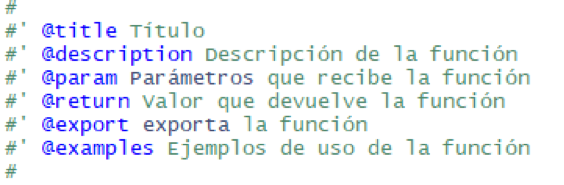
\includegraphics[scale=1]{Imagen_2}
    \caption{Ejemplo roxygen2   }
    \label{fig:roxygen}
\end{figure} 

Para ello se deben configurar las \textbf{Build Tools} de nuestro proyecto:

\begin{figure}[H]
    \centering
    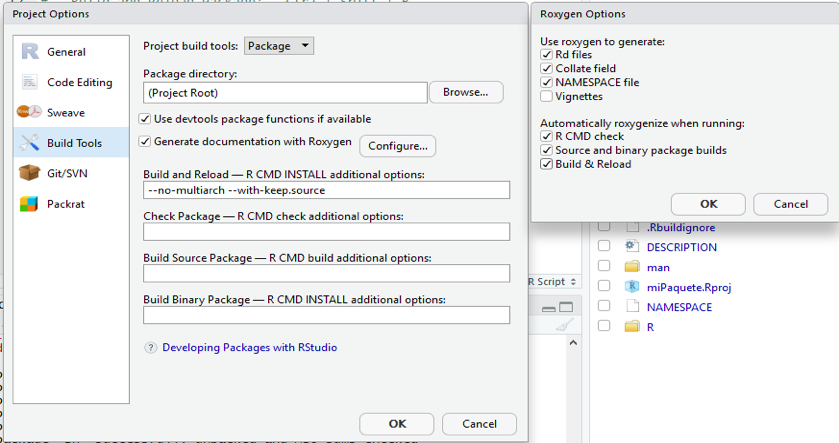
\includegraphics[scale=1]{Imagen_1}
    \caption{Configuraci\'on Build Tools }
    \label{fig:build_tools}
\end{figure} 

M\'as adelante se hablar\'a del uso del paquete \textbf{roxygen2} para generar la documentaci\'on del paquete

\subsubsection{Archivo DESCRIPTION}

En primer lugar, el archivo \textbf{DESCRIPTION} es lo que indica a R Studio que el directorio que lo
contiene es un paquete. Cuando se crea un proyecto e indicamos a R Studio que se va a
tratar de un paquete, este autom\'aticamente genera una plantilla del archivo \textbf{DESCRIPTION}
con los campos necesarios. De igual forma, si se crea el paquete haciendo uso de la herramienta \textbf{devtools}, se obtendr\'a
una plantilla similar.

\begin{figure}[H]
    \centering
    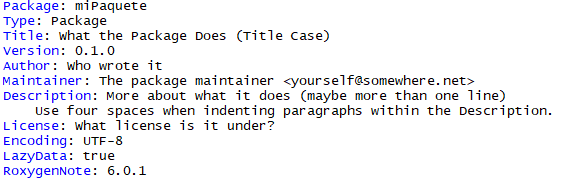
\includegraphics[scale=1]{pkge_metadata_1}
    \caption{Ejemplo Archivo DESCRIPTION }
    \label{fig:description}
\end{figure}

Este archivo usa un formato simple denominado \textit{Debian control format (DCF)} cuya estructura
es muy simple, cada l\'inea consiste en un campo y un valor separados por \enquote*{:}, cuando el valor
ocupa m\'as de una l\'inea hay que tabular las l\'ineas.

A parte de los campos de la plantilla existen otros m\'as a tener en cuenta como son \textbf{Imports}
y \textbf{Suggests}, ambos sirven para indicar las dependencias de nuestro paquete con respecto a otros.
Los principales campos de este archivo son: Package, Type, Title, Version, Author, Maintainer, Description y License.

La forma m\'as f\'acil de a\~nadir un paquete a \textbf{Imports} y \textbf{Suggests} es mediante el uso de
\textbf{devtools}, otra forma es haci\'endolo a mano en el archivo \textbf{DESCRIPTION}.

\begin{figure}[H]
    \centering
    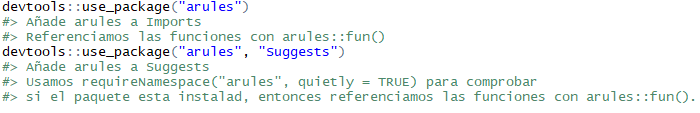
\includegraphics[scale=0.9]{pkge_metadata_6}
    \caption{Imports y Suggests con devtools }
    \label{fig:import_suggest}
\end{figure}

\subsubsection{Documentaci\'on de objetos}

En este caso se va a detallar la documentaci\'on de los distintos elementos que componen el
paquete.
Este tipo de documentaci\'on es accesible a trav\'es de \textbf{?} o \textbf{help()} y funciona como un
diccionario, permitiendo al usuario obtener informaci\'on sobre una funci\'on, paquete o conjunto
de datos.\\

\textbf{Crear la documentaci\'on}

Para crear esta documentaci\'on, lo primero que se debe hacer es a\~nadir comentarios
\textbf{roxygen} a los archivos \textbf{.R}, como, por ejemplo:

\begin{figure}[H]
    \centering
    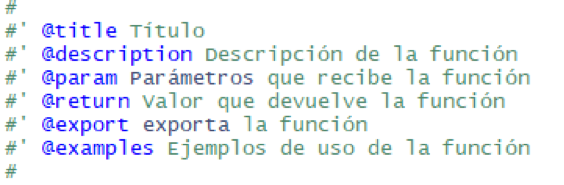
\includegraphics[scale=1]{Imagen_2}
    \caption{Ejemplo roxygen2   }
    \label{fig:roxygen2}
\end{figure} 

Una vez completado esto, presionamos \textbf{Ctrl/Cmd + Shift + B}, esto reconstruir\'a
completamente el paquete, actualizar\'a la documentaci\'on, reiniciar\'a R y recargar\'a \'el
paquete. \\

\textbf{Comentarios roxygen} \\
Estos comentarios comienzan con \textbf{\#'} y se colocan delante de cada funci\'on formando lo que
se llama un \textbf{bloque}. Estos bloques se dividen en \textbf{tags} (@NombreDelTag), el contenido de un
\textbf{tag} se extiende desde el final del nombre del tag hasta el inicio del siguiente o el final del
bloque.

Adem\'as, cada bloque incluye texto previo al primer tag, esto se denomina la introducci\'on y
se estructura de la siguiente forma:

\begin{itemize}
    \item La primera frase se corresponde con el t\'itulo de la documentaci\'on, es lo primero que
se ve cuando se consulta la ayuda de un paquete o funci\'on. Debe constar de solo
una l\'inea y acabar en punto.
    \item El segundo p\'arrafo es la descripci\'on, se muestra inmediatamente despu\'es del t\'itulo y
debe dar una breve descripci\'on de lo que hace la funci\'on.
    \item Por \'ultimo, el resto de p\'arrafos, si los hubiera, corresponden a una descripci\'on m\'as
detallada del funcionamiento de la funci\'on. Tambi\'en se puede usar el tag \textbf{@section}
para dividir los detalles de la funci\'on en distintas secciones.
\end{itemize}

El t\'itulo y la descripci\'on son obligatorios, mientras que los detalles son opcionales.
\textbf{Nota}: cada l\'inea de \textbf{roxygen} no debe superar los 80 caracteres y es recomendable tabular
las l\'ineas para facilitar la lectura.\\

\textbf{Documentando funciones} \\
Adem\'as del bloque introductorio y los tags ya mencionados, las funciones cuentan con una
serie de tags propios:
\begin{itemize}
    \item \textbf{@param} compuesto por un nombre y una descripci\'on. Sirve para describir los
par\'ametros de entrada de la funci\'on, su nombre, su tipo y para qu\'e se utilizan.
    \item \textbf{@examples} sirve para proveer c\'odigo en R que muestre un ejemplo de c\'omo funciona
la funci\'on. El c\'odigo debe funcionar sin errores. Esto es importante ya que muchos
usuarios miran primero los ejemplos.
    \item \textbf{@return} descripci\'on de la salida de la funci\'on.
\end{itemize}

\textbf{Documentando paquetes}\\
Se puede usar \textbf{roxygen} para crear una p\'agina de ayuda propia del paquete, no asociada a
una funci\'on en particular. Esta p\'agina es accesible mediante\\ \textbf{package?}\textit{nombreDelPaquete} y
puede ser usada para describir los componentes m\'as importantes del paquete o las
dependencias que tiene, por ejemplo.

En este caso, dado que no se corresponde con un objeto en concreto, se debe etiquetarlo
manualmente como \textbf{@docType package} y \textbf{@name} \textit{nombreDelPaquete} y poner un \textbf{NULL} al final.

\begin{figure}[H]
    \centering
    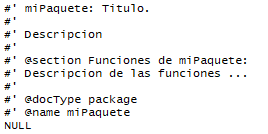
\includegraphics[scale=1]{od_1}
    \caption{Ejemplo documentaci\'on paquete }
    \label{fig:paquete}
\end{figure} 

\subsubsection{Datos externos}

Hay tres maneras principales de incluir datos en un paquete, dependiendo de qu\'e queramos
hacer con ellos o qui\'en debe usarlos:

\begin{itemize}
    \item Si se quiere almacenar datos binarios y que est\'en disponibles para los usuarios, se
deben poner en el directorio \textbf{data/}. Este es el mejor sitio para los datasets.
    \item Si lo que se quiere es almacenar datos de an\'alisis, pero que los dem\'as usuarios no
los tengan disponibles, se deben colocar en \textbf{R/sysdata.Rda}. En este caso es el mejor
sitio para los datos que necesiten nuestras funciones.
    \item Por \'ultimo, si queremos almacenar datos raw, se deben almacenar en el directorio
\textbf{inst/data}.
\end{itemize}

Si \textbf{DESCRIPTION} incluye LazyData: true, entonces los datasets se cargar\'an de forma
\enquote*{Lazy}. Es decir, que no ocupar\'an memoria hasta que se usen, \textbf{devtools::cr\'eate()} establece
\textbf{LazyData} a true autom\'aticamente.

\subsubsection{NAMESPACE}

El archivo \textbf{NAMESPACE} es muy importante en eñ paquete, ya que  ayuda a encapsular el paquete y que no falle por las dependencias que pueda tener de otros, ni
interfiera en otros que lo usen si lo actualizamos.

Como su nombre indica, \textbf{NAMESPACE} proporciona \enquote*{espacios para nombres}. Por ejemplo,
cuando se importan dos paquetes que ambos contienen una funci\'on con el mismo nombre,
se puede desambiguar con el operador \enquote*{::}. Por ejemplo, si se usan los paquetes \textit{plyr} ys
\textit{Hmisc}, ambos tienen la funci\'on \textbf{sumarize()}, por lo que, dependiendo de cu\'al se quiera usar,
se usar\'a \textbf{plyr::sumarize()} o \textbf{Hmisc::sumarize()}.

\textbf{NAMESPACE} hace el paquete autocontenido, tanto con los \textbf{Imports}, como con los
exports. Los \textbf{Imports}, definen c\'omo una funci\'on de un paquete encuentra una funci\'on de
otro. Los \textbf{exports}, ayudan a evitar los conflictos con otros paquetes especificando qu\'e
funciones se pueden usar fuera de nuestro paquete.\\

\textbf{El archivo NAMESPACE}

Cada l\'inea contiene una directriz: \textbf{S3method(), export(), exportClasses()}, adem\'as de otros.
Cada una de estas directivas describe un objeto de R, que nos indica si se exporta desde
el paquete para ser usado por los dem\'as o si se importa para usarlo de forma local.
En total hay ocho directrices. 

Cuatro de ellas describen las exportaciones:

\begin{itemize}
    \item \textbf{ export()}: exporta una funci\'on.
    \item \textbf{ exportPattern()}: exporta todas las funciones que coinciden con un patr\'on.
    \item \textbf{ exportClasses(), exportMethods()}: exporta las clases S4 y sus m\'etodos.
    \item \textbf{ S3method()}: exporta los m\'etodos de S3.
\end{itemize}

Y las cuatro restantes describen las importaciones:
\begin{itemize}
    \item \textbf{import()}: importa todas las funciones de un paquete.
    \item \textbf{importFrom()}: importa las funciones seleccionadas.
    \item \textbf{importClassesFrom(), importMethodsFrom()}: importa las clases S4 y sus
m\'etodos.
    \item \textbf{useDynLib()}: importa una funci\'on de C.
\end{itemize}

Generar el namespace con \textbf{roxygen2} es como generar la documentaci\'on para las funciones,
se usan los bloques y tags, a\~nadiendo los comentarios al \textbf{.R} correspondiente, se ejecuta
\textbf{devtools::document()} (o, \textbf{Ctrl + Shift +D}) y se comprueba que el archivo \textbf{NAMESPACE} se
haya modificado correctamente.\\

\begin{figure}[H]
    \centering
    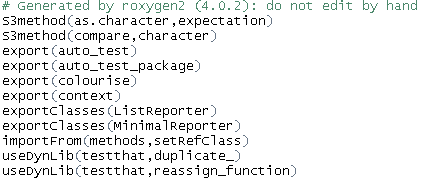
\includegraphics[scale=1]{namespace_2}
    \caption{Ejemplo de archivo NAMESPACE generado por roxygen2 }
    \label{fig:namespace}
\end{figure} 

\textbf{Exports}\\
Para que una funci\'on sea usable fuera de nuestro paquete debemos exportarla. Las funciones que se exporten deben estar documentadas.

\textbf{Imports}\\
\textbf{NAMESPACE} tambi\'en controla las funciones externas que pueden ser usadas en nuestro
paquete sin usar \enquote*{::}.

\subsection{Comprobando el paquete}

Una parte importante del desarrollo de un paquete es comprobar que el c\'odigo y la
documentaci\'on no presenten problemas, especialmente si se planea distribuir p\'ublicamente
el paquete. Para ello se tiene la herramienta que proporciona \textbf{devtools}, en concreto,
\textbf{devtools::check()} o, equivalentemente, \textbf{Ctrl + Shift + E} en R Studio.
Esta herramienta se encarga de que toda la documentaci\'on del paquete este actualizada, ya
que ejecuta \textbf{devtools::document()} de manera autom\'atica.

Encapsula el paquete antes de realizar las comprobaciones. Esto asegura que la
comprobaci\'on del paquete se hace desde un estado limpio ya que el encapsulamiento no
contiene ning\'un posible archivo temporal que se haya podido acumular y que pueda interferir
en las comprobaciones.\\

La mejor forma, aunque tediosa, de comprobar el paquete es la siguiente:

\begin{itemize}
    \item Ejecutar \textbf{devtools::check()} o \textbf{Ctrl + Shift + E} en R Studio.
    \item Arreglar el primer problema.
    \item Repetir los dos anteriores hasta que no haya m\'as problemas.
\end{itemize}

\textbf{devtools::check()} devuelve tres tipos de problemas distintos:

\begin{itemize}
    \item \textbf{Error}: Problema grave que deber ser arreglado, aunque no se planee subir el paquete a CRAN.
    \item \textbf{Warning}: Problema medio que debe ser arreglado en caso de que se planee subir el paquete a CRAN.
    \item \textbf{Note}: Problema medio que se deber\'ia arreglar en caso de querer subir el paquete a CRAN incluso si se trata de un falso positivo.
\end{itemize}


\subsection{Liberando el paquete}

Si se quiere que el paquete tenga cierta trascendencia en la comunidad de R, es necesario subirlo a CRAN, ya que la mayor\'ia de usuarios descargan e instalan sus paquetes desde CRAN.
A continuaci\'on, se detallar\'an las buenas pr\'acticas a la hora de distribuir el paquete a en CRAN. \\

\textbf{Comentarios CRAN}\\
Debemos recordar que CRAN est\'a compuesto por voluntarios que dedican parte de su tiempo
libre a revisar los paquetes que se suben, por tanto, cuanto m\'as f\'acil se les haga el trabajo,
m\'as posibilidades hay de que el paquete sea aceptado sin ning\'un problema.
Por ello, es recomendable a\~nadir al paquete una serie de comentarios que faciliten la tarea de revisi\'on, estos comentarios ir\'an en un archivo llamado \textbf{cran-comments.md}.

\begin{figure}[H]
    \centering
    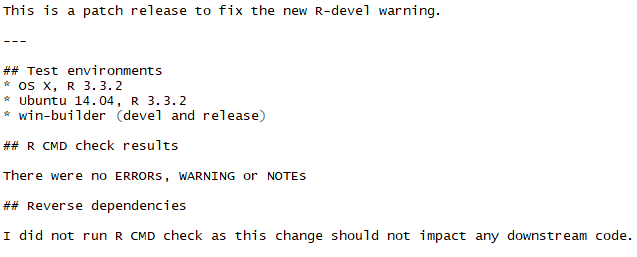
\includegraphics[scale=0.9]{rp_6}
    \caption{Comentarios CRAN}
    \label{fig:comentarios}
\end{figure} 
\begin{itemize}

    \item \textbf{Test environments}: indica en qu\'e plataformas se ha comprobado el paquete.
    \item \textbf{Check results}: contendr\'a una lista de errores, advertencias o notas.
    \item \textbf{Reverse dependencies}: sirve para indicar que si hay errores de dependencias con
otros paquetes en el caso de que se este  subiendo una nueva versi\'on del paquete y los cambios hayan provocado errores en las dependencias con otros paquetes.
\end{itemize}

\textbf{Las pol\'iticas en CRAN}\\
Existen ciertas pol\'iticas que debemos cumplir a la hora de subir el paquete a CRAN, estas son comprobadas manualmente. Algunos problemas comunes son:
\begin{itemize}
    \item Ausencia del email del mantenedor del paquete. 
    \item Es importante dejar claro los propietarios del copyright y si se ha usado c\'odigo externo, comprobar que la licencia es compatible.
    \item Paquetes que no funcionan en al menos dos plataformas no ser\'an considerados.
    \item No hacer cambios externos sin permiso del usuario: cambiar opciones, instalar paquetes, abrir software externo, cerrar R, etc.
    \item No subir actualizaciones del paquete muy frecuentemente. La pol\'itica sugiere hacerlo cada 1 o 2 meses como mucho.
\end{itemize}

\textbf{Archivos importantes}\\
Una vez que el paquete ya est\'a listo para subirlo, se deben  tener en cuenta dos archivos importantes m\'as,\textbf{ README.md}, el cual proporciona una descripci\'on del paquete y su
funcionamiento y uso, y \textbf{NEWS.md}, el cual describe los cambios con respecto a la versi\'on anterior del paquete. Dado que estos dos archivos no son soportados por CRAN no
hay que a\~nadirlos a la hora de construir el paquete
\begin{center}
    \textbf{devtools::use\_build\_ignore("NEWS.md")
    devtools::use\_build\_ignore("README.md")}
\end{center}


\textbf{Lanzamiento}

Lleg\'o la hora de construir el paquete y subirlo a CRAN. Para construir el paquete
usamos \textbf{devtools::release()}. Esto se encarga de volver a comprobar el paquete una \'ultima
vez y nos hace una serie de preguntas acerca de buenas pr\'acticas a modo de comprobaci\'on,
\textbf{devtools::release()}, autom\'aticamente, sube el paquete a CRAN.
Una vez subido, los voluntarios de CRAN comprobar\'an el paquete y
devolver\'an los resultados.
En caso de fallo, se deben resolver los problemas, y ejecutar \textbf{devtools::submit\_cran()} para evitar contestar de nuevo todas las preguntas de \\
\textbf{devtools::release()}.

\newpage
% \section{Motivaci\'on}

\newpage
\thispagestyle{empty}
\mbox{}

\newpage
% \section{Objetivos}

\newpage
\thispagestyle{empty}
\mbox{}

\newpage
% \section{Estudio del arte}

\newpage
\thispagestyle{empty}
\mbox{}

\newpage
\subsubsection{Descripci\'on} 

El primer paso del desarrollo de este projecto consiste en la creaci\'on de una peque\~na libreria de funciones
orientadas a aplicar la l\'ogica de simplificaciones a los conjuntos de reglas con los se trabaja. Como 
puede ser la composici\'on de reglas, la reducci\'on, la uni\'on y la simplificaci\'on.

Estas funciones, adem\'as de formar parte de los algoritmos desarrollados, nos permiten reducir el n\'umero de 
reglas y la complejidad de las mismas con el objetivo de minimizar los requisitos computacionales y de tiempo
necesarios para la ejecuci\'on de los algoritmos. As\'i como mantener limpio el c\'odigo de los algoritmos

Esta l\'ogica de simplificaciones esta basada en los axiomas de Amstrong.

\textbf{Axioma de Reflexividad}

\begin{center}
    \(Y \subseteq X \implies X \to Y \)
\end{center}

\textbf{Axioma de Aumentatividad}

\begin{center}
    \(X \to Y \implies XZ \to YZ \) para cualquier Z
\end{center}

\textbf{Axioma de Transitividad}

\begin{center}
    \(X \to Y \wedge Y \to Z \implies X \to Z \)
\end{center}

Por ello, la libreria contiene definida una funci\'on por cada regla de la l\'ogica de implicaciones. A continuaci\'on se detallar\'an las mas relevantes, como son la simplificaci\'on, la rsimplificaci\'on, la ssimplificaci\'on o la uni\'on de reglas.\\

\textbf{Uni\'on}\\
La uni\'on de reglas parte de la base de que si tenemos dos reglas (\(X \to Y , X \to Z\)) cuyos antecedentes son iguales, podemos inferir una nueva regla que tendra como antecedente el mismo y como consecuente la union de los consecuentes de ambas reglas, es decir:

\begin{center}
    \(X \to Y \wedge X \to Z \implies X \to YZ \)
\end{center}

\lstinputlisting{r_code/composition.R}

\textbf{Simplificaci\'on}\\
La simplificaci\'on de reglas se basa en que si disponemos de dos reglas \\ (\(X \to Y , U \to V\)) cuyos antecedentes no son disjuntos (\(X \subseteq U\)) y se cumple que el antecedente y el consequente de una de ellas si son disjuntos (\(X \cap Y \neq \emptyset\)) podemos simplificar la otra regla de la siguiente forma:

\begin{center}
    \(Siendo \ X \to Y \ y \ U\to V \ dos \ reglas \ | \ X \subseteq U \wedge X \cap Y \neq \emptyset \implies (U - Y) \to (U - Y)\)
    % \(U \to V \implies (U - Y) \to (U - Y) \)
\end{center}

\lstinputlisting{r_code/simplification.R}

\textbf{Rsimplificaci\'on}\\

\lstinputlisting{r_code/rsimp.R}

\textbf{Simplificaci\'on fuerte}\\

\lstinputlisting{r_code/ssimp.R}

\textbf{Lsimplificaci\'on}\\

\lstinputlisting{r_code/lsimp.R}


\section{Algoritmos}
\subsection{IO library}

\lstinputlisting{I_O.R}

%Estudio de FCA
\subsection{FCA}





%Estructura de datos
\subsection{Estructura de datos}

Cuando se comienza a realizar un algoritmo que se necesita que 
sea r\'apido y est\'e optimizado, una de las cosas m\'as importantes 
es decidir qu\'e estructura de datos se va a utilizar.
Ya que, dependiendo de qu\'e queramos hacer, elegir bien, nos puede 
ayudar a ganar tiempo en el algoritmo.
\\
\\
Por ello, para la gran mayor\'ia de algoritmos que vamos a realizar 
en este TFG se va a utilizar la estructura ItemMatrix, perteneciente al paquete 
arules.

 %Librería básica
\subsection{Librer\'ia b\'asica para sistemas de implicaciones}


%Conjuntos aleatorios
\subsection{Random Implications Generator}


%Data mining
\subsection{Data mining}




\newpage
\thispagestyle{empty}
\mbox{}

\newpage
\section{Claves y generadores minimales}

\subsection{Labeled Closed Set}

\textbf{Descripci\'on} 

En AFC los generadores minimales y sus cerrados son elementos esenciales en el ret\'iculo de conceptos  que se obtiene a partir de la relaci\'on binaria de entrada. 

Ser\'ia el equivalente al c\'alculo de las claves minimales. El cerrado de las claves minimales es el conjunto de atributos del dataset. 

Ahora aparecen muchos cerrados y tenemos que calcular sus generadores minimales. Es un problema catalogado como \enquote*{hard} (exponencial en n\'umero de atributos).

Existen algunos algoritmos que  calculan generadores minimales pero no implementados en R y no est\'an basados directamente en la l\'ogica. El director del proyecto no ha realizado comparativas en este \'ambito con los otros algoritmos por la no disponibilidad de ellos.



Dados un conjunto de atributos \(M\) y un sistema implicacional \(\Sigma\) sobre \(M\), este algoritmo desarrollado por P. Cordero et al. \cite{LCS} calcula los generadores minimales haciendo uso del concepto de \textit{Labeled Closed Set}, que se basa en que si tenemos un conjunto \(A \subseteq M\), \(A\) es generador minimal si \(X^+_{\Sigma} = A^+_{\Sigma}\) implica que \(X = A\) para todo  \(X \subseteq A\). 

Podemos definir el conjunto de \textit{Labeled Closed Sets} con respecto a \(\Sigma\) como:
\begin{center}
    \(\{<C,mg(C)> | \ C \subseteq M, \ C^+_{\Sigma} = C \}\)\\
     \(donde \ mg(C) = \{D \subseteq M \ | \ D \ es \ generador \ minimal \ y \ D^+_{\Sigma} = C \}\)
\end{center}

De esta forma, al calcular el conjunto de \textit{Labeled Closed Sets} con el siguiente algoritmo, autom\'aticamente se calculan los generadores minimales.\\

\IncMargin{1em}
\begin{algorithm}[H]
    \SetKwFunction{LabeledClosedSets}
    \SetAlgoLined
    % \LinesNumbered
    \DontPrintSemicolon
    \SetKw{KwOr}{or}
    \KwIn{  
        $M$, the set of all attributes\\
        $ \ \ \ \ \ \ \ \ \ \ \ \ Label$, A structure to build a minimal generator\\
        $ \ \ \ \ \ \ \ \ \ \ \ \ Cicerone$, A structure to build a closed set\\
        $ \ \ \ \ \ \ \ \ \ \ \ \ \Sigma$, an implicational system on $M$
    }
    \KwOut{The set of Labeled Closed Sets}
    \Begin{
        \Repeat{$\Sigma = \Gamma$} {
            \ $\Sigma = \Gamma$\;
            \ $\Gamma = \emptyset$\;
            \For{$A \to B \in \Sigma $}{
                \If{$A \subseteq Cicerone$}{
                    \ $Cicerone := Cicerone \cup {B}$
                }\uElseIf{$B \not\subseteq Cicerone$}{
                    \ $\Gamma := \Gamma \cup \{A \setminus Cicerone \to B \setminus Cicerone\}$
                }
            }
        }
        \ $M := M \setminus Cicerone$\;
        \ $Mnl = \{A \subseteq M \ | \ A \to B \in \Gamma \ for \ some \ B \subseteq M \ and$\; 
        \ $ \ \ \ \ \ \ \ \ \ \ \ \ C \subseteq A \ implies \ C = A \ for \ all \ C \to D \in \Gamma\}$\;
        \ $NC := \{ X \subseteq M \ | \ A \not\subseteq X \ for \ all \ A \in Mnl \}$\;
        \ $LCS := \emptyset$\;
        \ForEach{$X \in NC$}{
            \ $LCS := LCS \cup \{\langle Cicerone \cup X, \{Label \cup X\}\rangle\}$
        }
        \ForEach{$A \in Mnl$}{
            \ $LCS := LCS \cup \LabeledClosedSets{$ M,Label \cup A,Cicerone \cup A, \Gamma $}$
        }
        \Return $LCS$
    }%end beginre
    \caption{LabeledClosedSets algorithm}\label{alg:3}
\end{algorithm}\DecMargin{1em}
\newpage

\textbf{C\'odigo} 
\lstinputlisting{r_code/labeled.closed.set.R}
\textbf{Ejemplo} 

A continuaci\'on, se muestra un peque\~no ejemplo de ejecuci\'on del algoritmo. Para ello se parte del conjunto de atributos \(M\) y del conjunto de implicaciones \(\Gamma\) que se puede ver en la imagen \ref{fig:lcs_4}.
\begin{figure}[H]
    \centering
    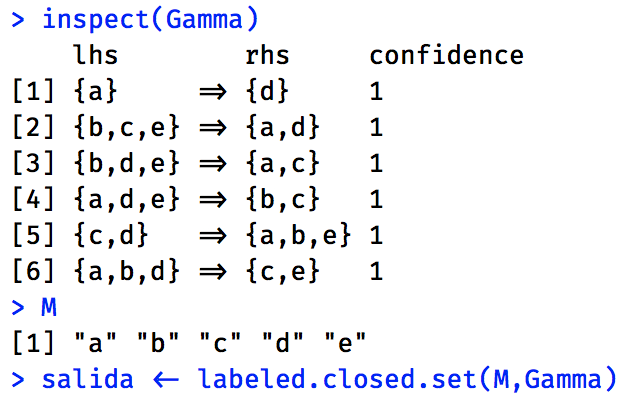
\includegraphics[scale=0.75]{lcs_4}
    \caption{Ejemplo LCS 1}
    \label{fig:lcs_4}
\end{figure} 
\newpage
Aqu\'i se puede ver el resultado:
\begin{figure}[H]
    \centering
    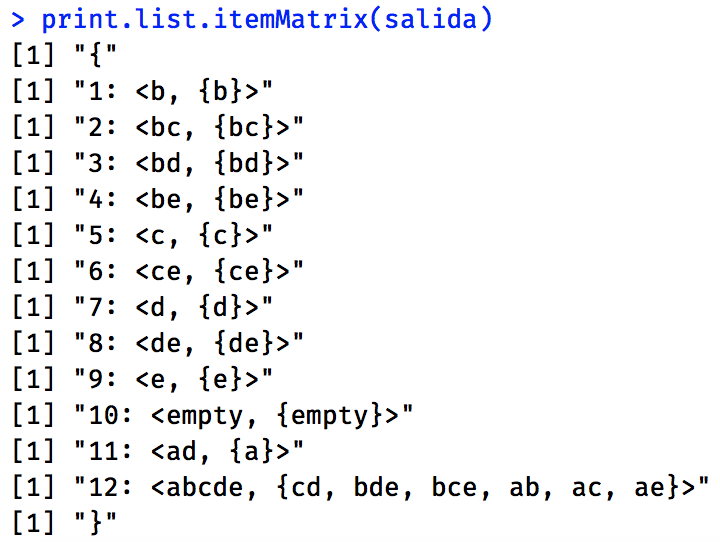
\includegraphics[scale=0.75]{lcs_3}
    \caption{Ejemplo LCS 2}
    \label{fig:lcs_3}
\end{figure}

Como puede verse, por ejemplo, el cerrado 12 tiene como generadores minimales \{cd, bde, bce, ab, ac, ae\}.

Y aqu\'i el resultado que se obtendr\'ia si se usa la otra versi\'on del algoritmo:
\begin{figure}[H]
    \centering
    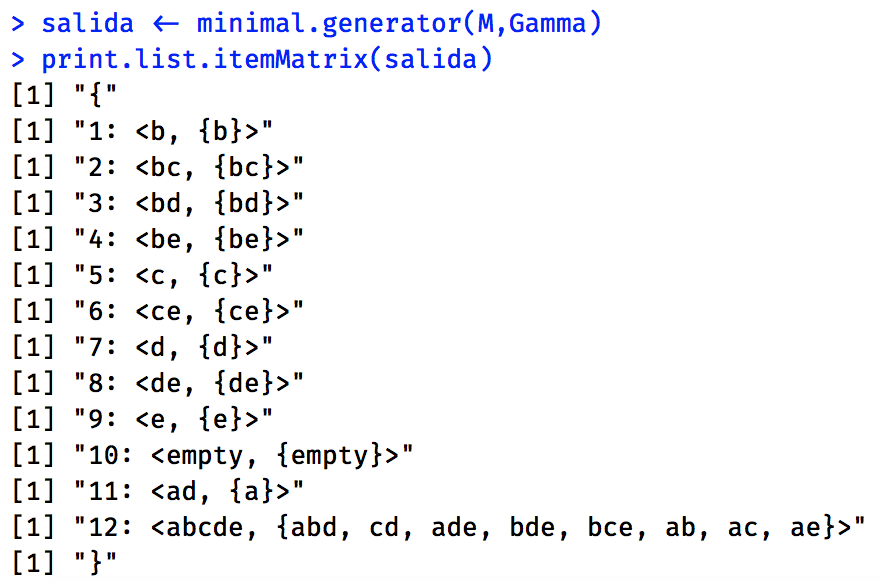
\includegraphics[scale=0.75]{lcs_5}
    \caption{Ejemplo LCS 3}
    \label{fig:lcs_5}
\end{figure}
\newpage
\textbf{Comparativa/Versiones}  
\newpage

\subsection{Claves minimales}

\subsubsection{Descripci\'on} 
\subsubsection{Contexto NO} 
\newpage
\subsubsection{C\'odigo} 
\lstinputlisting{reduction.method.R}
\newpage
\subsubsection{Ejemplo} 
\subsubsection{Comparativa/Versiones}  

\newpage
\section{C\'alculo de bases}

\subsection{Base Directa \'Optima}

\subsubsection{Descripci\'on} 

% \textbf{Direct-optimal basis computation by means of the fusion of Simplification rules, E. Rodr ́ıguez-Lorenzo et.al., Last review Discrete Appl. Math (2017)}

Una vez que hemos conseguido un algoritmo para el c\'alculo del cierre eficiente y optimizado, el siguiente paso para reducir el coste del c\'alculo del cierre es optimizar todo lo posible el sistema implicacional de entrada. Es aqu\'i donde entran en juego nuevos conceptos como son, por ejemplo, el de base directa \'optima.

K. Bertet \cite{BERTET20102155} propuso la llamada base directa \'optima como primera aproximaci\'on para reducir el coste del c\'alculo del cierre. Mientras que  K. Adaricheva \cite{Adaricheva} propuso la llamada D-Base como un subconjunto de la base directa \'optima. Esto supon\'ia un problema abierto: mejorar el c\'alculo de estas bases (o algo similar) para reducir el coste del c\'alculo del cierre en consecuencia.

La importancia del c\'alculo de bases directas de sistemas implicacionales ha sido remarcada por diferentes autores en \'areas diferentes ya que su uso es crucial en problemas donde se requiere el c\'alculo de gran cantidad de cierres. Por lo tanto, cuanto m\'as eficiente sea el c\'alculo de estas bases, mejor rendimiento tendr\'an los m\'etodos de resoluci\'on de esos problemas. 

A continuac\'on se van a detallar algunos de estos conceptos.\\


\textbf{Base}

Un sistema implicacional \( \Sigma \) se dice que es:
\begin{itemize}
    \item Una base minimal cuando,  \( para \ todo \ A \to B \in \Sigma \ se \ tiene \ que \ \Sigma \setminus \{A \to B\} \not\equiv \Sigma\)

    \item Una base m\'inima cuando,  \( para \ todo \ \Sigma' \equiv \Sigma \ se \ tiene \ que \ |\Sigma| \leq |\Sigma'|\)

    \item Una base \'optima cuando,  \( para \ todo \ \Sigma' \equiv \Sigma \ se \ tiene \ que \ \|\Sigma\| \leq \|\Sigma'\| \\ donde \ \|\Sigma\| = 
    \sum_{\substack{A \to B \in \Sigma}} (|A|+|B|) \).
\end{itemize}

\textbf{Directo}

Un sistema implicacional \( \Sigma \) se dice que es directo cuando, \( para \ todo \ X \subseteq S \ se \ tiene \ que \\ X^+_{\Sigma} =  X \cup \{ B | A \to B \in \Sigma \ para \ algun \ A \subseteq X \} \). Esto se traduce en que se puede calcular el cierre de un conjunto de atributos con una sola pasada y que ninguna de las implicaciones puede ser eliminada sin perder esta propiedad.

Por tanto, ya se est\'a en condiciones de conocer qu\'e es una base directa \'optima.\\

El teorema 2 de \cite{DO2} nos dice que:

Para cualquier sistema impicacional \(\Sigma\), existe un \'unica base directa \'optima \(\Sigma_{DO}\) tal que \(\Sigma \equiv \Sigma_{DO} \).\\

Como soluci\'on al c\'alculo de bases directas \'optimas se ha implementado el algoritmo desarrollado por  E. Rodr\'iguez-Lorenzo et al. \cite{DO2}, llamado [SLgetdo] en el cu\'al se aplican las reglas de L\'ogica de Simplificaciones \(\textbf{SL}_{FD}\).\\

\IncMargin{1em}
\begin{algorithm}[H]
    \SetAlgoLined
    % \LinesNumbered
    \DontPrintSemicolon
    \SetKw{KwOr}{or}
    \KwIn{ 
        $\Sigma$, an implicational system on $S$
    }
    \KwOut{A simplified implicational system $ \Sigma_{s} $ that is equivalent to $\Sigma$}
    \Begin{
        \ $ \Sigma := \{ A \to B \setminus A \ | \ A  \to B \in \Sigma, \ B \not\subseteq A \}$\;
        \Repeat{$ \Sigma_{s} = \Sigma $} {
            \ $\Sigma_{S} = \Sigma$\;
            \ $\Sigma := \emptyset$\;
            \ForEach{$A \to B \in \Sigma_{s} $}{
                \ $\Gamma = \emptyset$\;
                \ForEach{$C \to D \in \Sigma $}{
                    \lIf{$C \subseteq A \subseteq (C \cup D) \ or \ A \subseteq C \subseteq (A \cup B)$}{
                        \ $A := A \cap C ; \ B := B \cap D$ 
                    }\Else{
                        \lIf{$A \subset C$}{
                            \If{$D \not\subseteq B$}{
                                \ $ add \ C \setminus B \to D \setminus B \ to \ \Gamma$ 
                            }   
                        }\Else{
                            \If{$C \subset A$}{
                                \ $ A := A \setminus D ; \ B := B \setminus D$ 
                            } 
                            \ $\Gamma := \Gamma \cup \{C \to D \} \cup $
                        }
                    }
                }
                \lIf{$B = \emptyset$}{
                    \ $\Sigma := \Gamma$
                }\lElse{
                    \ $\Sigma := \Gamma \cup \{A \to B\}$
                }
            }
        }
        \Return $\Sigma_{s}$
    }%end beginre
    \caption{Simplify}\label{alg:4}
\end{algorithm}\DecMargin{1em}

% Add-sSimp

% \IncMargin{1em}
% \begin{algorithm}[H]
%     \SetAlgoLined
%     % \LinesNumbered
%     \DontPrintSemicolon
%     \SetKw{KwOr}{or}
%     \Begin{
%         \If{$A \not\subseteq C \ and \ B \cup C \neq \emptyset \neq D \setminus (A \cup B)$}{
%             \ $E := A \cup (C \setminus B)$ \;
%             \ $F := D \setminus (A \cup B)$ \;
%             \ForEach{$X \to Y \in \Sigma $}{
%                     \If{$X \subseteq E$}{
%                         \lIf{$C \subseteq Y$}{
%                             \Return $\emptyset$
%                         }\Else{
%                             \ $E := E \setminus Y$\;
%                             \ $F := F \setminus Y$\;
%                         } 
%                     }
%             } 
%             \Return $\{E \to F\}$
%         }\lElse{
%             \Return $\emptyset$
%         }
%     }%end beginre
%     \caption{Add-sSimp}\label{alg:5}
% \end{algorithm}\DecMargin{1em}

.

\IncMargin{1em}
\begin{algorithm}[H]
    \SetKwFunction{Simplify}{Simplify}
    \SetKwFunction{Ssimp}{Add-sSimp}
    \SetAlgoLined
    % \LinesNumbered
    \DontPrintSemicolon
    \SetKw{KwOr}{or}
    \KwIn{ 
        $\Sigma$, an implicational system 
    }
    \KwOut{The equivalent direct-optimal implicational system $ \Sigma_{do} $}
    \Begin{
        \ $ \Sigma := \Simplify{$\Sigma$}$\;
        \Repeat{$ \Sigma_{do} = \Sigma $} {
            \ $\Sigma_{do} = \Sigma$\;
            \ $\Sigma := \emptyset$\;
            \ForEach{$A \to B \in \Sigma_{do} $}{
                \ $\Gamma = \emptyset$\;
                \ForEach{$C \to D \in \Sigma $}{
                    \lIf{$C \subseteq A \subseteq (C \cup D) \ or \ A \subseteq C \subseteq (A \cup B)$}{
                        \ $A := A \cap C ; \ B := B \cap D$ 
                    }\Else{
                        \lIf{$A \subseteq C$}{
                            \If{$D \not\subseteq B$}{
                                \ $ add \ C \setminus B \to D \setminus B \ to \ \Gamma$ 
                            }   
                        }\Else{
                            \If{$C \subseteq A$}{
                                \ $ A := A \setminus D ; \ B := B \setminus D$ 
                            } 
                            \ $\Gamma := \Gamma \cup \{C \to D \} \cup \Ssimp{$A \to B, \ C \to D, \ \Sigma$} \cup \Ssimp{$C \to D, \ A \to B, \ \Sigma$}$
                        }
                    }
                }
                \lIf{$B = \emptyset$}{
                    \ $\Sigma := \Gamma$
                }\lElse{
                    \ $\Sigma := \Gamma \cup \{A \to B\}$
                }
            }
        }
        \Return $\Sigma_{do}$
    }%end beginre
    \caption{SLgetdo algorithm}\label{alg:6}
\end{algorithm}\DecMargin{1em}

Una primera aproximaci\'on  fue el algoritmo desarrolado tambi\'en por E. Rodr\'iguez-Lorenzo et al. \cite{doSimp}, llamado doSimp tambi\'en basado en la L\'ogica de Simplificaciones, aplicando la simplificaci\'on Si-Eq y la composici\'on Co-Eq para simplificar el sistema implicacional, sSimp para completarlo y rSi-Eq y Co-Eq para optimizar el resultado final. Este primer algoritmo no se ha implementado en el proyecto ya que SLgetdo lo mejora, reduciendo el n\'umero de pasos a dos, as\'i como el tama\~no de las bases directas generadas hasta alcanzar la \'optima.
\newpage
\subsubsection{C\'odigo} 
\lstinputlisting{r_code/DO_IS.R}
\newpage
\lstinputlisting{r_code/simplify.R}
\newpage
\subsubsection{Ejemplo} 
% \textbf{[este ejemplo no me gusta, tiene vacios a la derecha.... y luego la base directa normalemente tiene mayor longitud. igual este ejemplo es de los que no va....¿¿??]}
A continuaci\'on, se muestra un ejemplo del c\'alculo de una base directa \'optima a partir del siguiente conjunto de implicaciones: 
\begin{figure}[H]
    \centering
    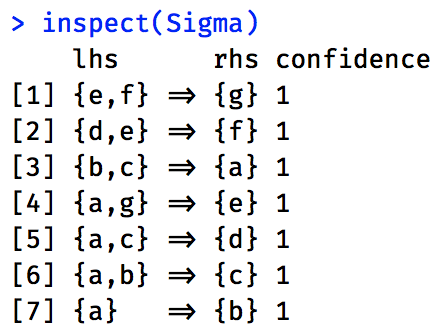
\includegraphics[scale=0.75]{SLgetDO1}
    \caption{Ejemplo SLgetdo 1}
    \label{fig:SLgetDO1}
\end{figure} 

Aqu\'i se puede ver el resultado:
\begin{figure}[H]
    \centering
    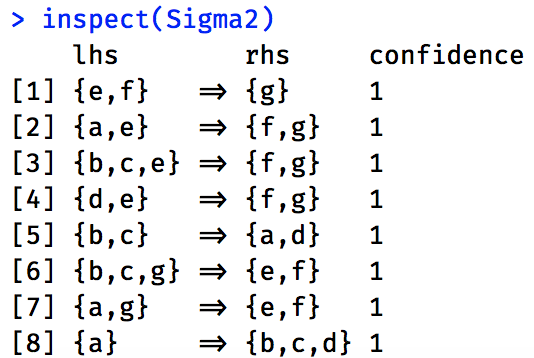
\includegraphics[scale=0.75]{SLgetDO2}
    \caption{Ejemplo SLgetdo 2}
    \label{fig:SLgetDO2}
\end{figure} 
Y, como era de esperar, el hecho de usar una base directa \'optima para el c\'alculo del cierre reduce consideradamente los tiempos de ejecuci\'on incluso en ejemplos tan peque\~nos como este, donde el c\'alculo es practicamente inmediato.\\

Se parte del conjunto de atributos \(\{c,f,g\}\)

\begin{figure}[H]
    \centering
    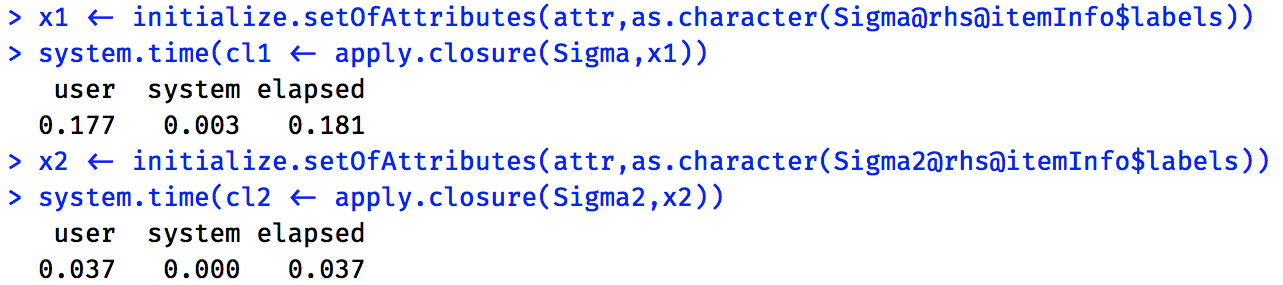
\includegraphics[scale=0.75]{SLgetDO4}
    \caption{Comparativa del c\'alculo del cierre a partir de una base DO}
    \label{fig:SLgetDO4}
\end{figure}

Y como se puede ver, el resultado es el mismo:
\begin{figure}[H]
    \centering
    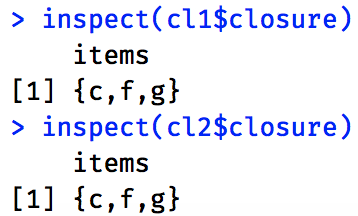
\includegraphics[scale=0.75]{SLgetDO5}
    \caption{Comparativa del c\'alculo del cierre a partir de una base DO 2}
    \label{fig:SLgetDO5}
\end{figure}

Esta reducci\'on de tiempo se acent\'ua conforme crece el tama\~no del conjunto de implicaciones.

Si se tiene en cuenta que para resolver determinados problemas, el c\'alculo de multitud de cierres (del orden de millones) es parte fundamental \cite{Adaricheva}, el impacto de cualquier peque\~na mejora en el c\'alculo de cada uno de esos cierres, puede suponer una diferencia abismal. De ah\'i radica la importancia de este algoritmo.

% \subsubsection{Comparativa/Versiones}  
\newpage

\subsection{D-Base}

\textbf{Descripci\'on} 

% \textbf{Motivation
% D-basis: Ordered direct implicational basis of a finite closure system, K. Adaricheva, et.al., Discrete Applied Mathematics, 161 (6): 707-723, 2013
% Compromise between the size of the implicational set and the efficiency of its management
% }

Este algoritmo se desarroll\'o por E. Rodr\'iguez-Lorenzo et al. en \cite{DBasis} con el objetivo  de reducir el coste computacional del c\'alculo del cierre haciendo uso del concepto de D-Base presentado por K. Adaricheva \cite{Adaricheva}.\\

\IncMargin{1em}
\begin{algorithm}[H]
    \SetKwFunction{Add}{Add}
    \SetKwFunction{MinimalCovers}{MinimalCovers}
    \SetKwFunction{MinGen}{$MinGen_{0}$}
    \SetKwFunction{OrderedComp}{OrderedComp}
    \SetAlgoLined
    % \LinesNumbered
    \DontPrintSemicolon
    \SetKw{KwOr}{or}
    \KwIn{ 
        $\Sigma$, an implicational system on $M$ 
    }
    \KwOut{The D-basis $ \Sigma_{D} $ on $M$}
    \Begin{
        \ $MinGen = \MinGen{$M, \ \Sigma $}$\;
        \ $C := \emptyset$\;
        \ForEach{$\langle a,mg(C)\rangle \in MinGen $}{
            \ForEach{$a \in C $}{
                \ $C := \Add{$\langle a,mg(C)\rangle,C$}$
            }
        }
        \ $\Sigma_{D} := \emptyset$ \;
        \ForEach{$\langle a,mg_{a}\rangle \in C $}{
            \ $mg_{a} := \MinimalCovers{$mg_{a}$}$\;
            \ForEach{$g \in ,mg_{a} $}{
                $\Sigma_{D} : = \Sigma_{D} \cup \{g \to a\}$
            }
        }
        \OrderedComp{$\Sigma_{D}$}\;
        \Return $\Sigma_{D}$
    }%end beginre
    \caption{D-basis algorithm}\label{alg:7}
\end{algorithm}\DecMargin{1em}
\bigskip

Antes de entrar en el concepto de D-Base, se detallar\'an otros conceptos con el fin de entrar en contexto.\\

Se parte de un conjunto de implicaciones \( \Sigma \) y un conjunto de atributos \( M \).\\

\textbf{Operador de cierre at\'omico}\\
Se parte de que \(\Sigma\) cumple las siguientes propiedades:
\begin{itemize}
    \item \(\oslash^+_{\Sigma} = \oslash\), es decir, el cierre del vac\'io con respecto a \(\Sigma\) es el vac\'io.
    \item \(\forall x,y \in M, \{x\}^+_{\Sigma} = \{y\}^+_{\Sigma} \implies x = y\)
\end{itemize}
Se define el operador de cierre at\'omico como: 
\begin{center}
    \((-)^*_{\Sigma}::2^M \to 2^M \) \\
    \(X^*_{\Sigma} = \cup_{\substack{x \in X}} \{x\}^+_{\Sigma}, \ \forall \ X \subseteq M \)
\end{center}


\textbf{Covers}\\
Sea \(X \subseteq M\) y \(x \in X\), se dice que \(X\) es un cover de \(x\) si \(x \in X^+_{\Sigma} \setminus X\), denotado por \(x \sim X\)

\textbf{Propers covers} \\
Sea \(X \subseteq M\) y \(x \in X\), se dice que \(X\) es un proper cover de \(x\) si \(x \in X^+_{\Sigma} \setminus X^*_{\Sigma}\), denotado por \(x \dot\sim X\)

\textbf{Minimals propers covers}\\
Sea \(X \subseteq M\) y \(x \in X\), se dice que \(X\) es un minimal proper cover de \(x\) si se cumple que:
\begin{itemize}
    \item \(x \dot\sim X\)
    \item \(x \dot\sim Z\) y \(Z \subseteq X^*_{\Sigma} \implies X \subseteq Z\)
\end{itemize}

\textbf{D-Base}\\
Podemos definir la D-Base para \(\Sigma\) como el par \(<\Sigma_a, \Sigma_n>\), donde:

\begin{itemize}
    \item \(\Sigma_a = \{y \to x \ | \ y \in M, \ x \in X^+_{\Sigma}, \ x \neq y \} \)
    \item \(\Sigma_n = \{X \to x \ | \ X \subseteq M, \ x \in X, \ X \ minimal \ proper \ cover \ de \ x\} \)

\end{itemize}

\textbf{Teorema}(\cite{Adaricheva})\\
Sea \(\Sigma\) un sistema implicacional. Si \(<\Sigma_a, \Sigma_n>\) es D-Base de \(\Sigma\) y \(\Sigma_d = \Sigma_a\cup \Sigma_n\) de forma que las implicaciones de \(\Sigma_a\) aparecen antes que las de \(\Sigma_n\), entonces \(\Sigma_d\) es una base ordenada directa de forma que \(\Sigma_d \equiv \Sigma\).

De este teorema radica la importancia de tener un algoritmo para el c\'alculo de la D-Base de un sistema implicacional \(\Sigma\), ya que a partir de esta, se podr\'a obtener una base ordenada directa, que como ya se ha dicho con anterioridad, permite que el c\'alculo del cierre de \(\Sigma\) sea mucho m\'as r\'apido y eficiente.\\


\newpage 
\textbf{C\'odigo} 
\lstinputlisting{r_code/d.basis.R}
\newpage
\textbf{Ejemplo}

A continuaci\'on, se muestra un peque\~no ejemplo de ejecuci\'on del algoritmo. Para ello, se parte del conjunto de atributos \(M\) y del conjunto de implicaciones \(\Gamma\) que se puede ver en la imagen \ref{fig:dbasis_2}.
\begin{figure}[H]
    \centering
    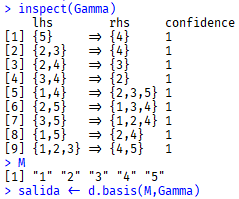
\includegraphics[scale=1]{dbasis_2}
    \caption{Ejemplo D-Base 1}
    \label{fig:dbasis_2}
\end{figure} 
Aqu\'i se puede ver el resultado:
\begin{figure}[H]
    \centering
    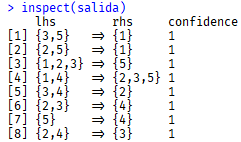
\includegraphics[scale=1]{dbasis_3}
    \caption{Ejemplo D-Base 2}
    \label{fig:dbasis_3}
\end{figure} 
Aunque el ejemplo expuesto tiene un conjunto reducido de implicaciones y atributos, se puede apreciar la mejora de rendimiento a la hora del c\'alculo del cierre si se hace sobre una base, en comparaci\'on a si se hace con el conjunto de implicaciones inicial.
\begin{figure}[H]
    \centering
    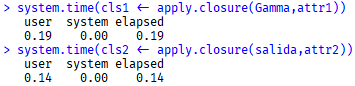
\includegraphics[scale=1]{dbasis_4}
    \caption{Comparativa de c\'alculo del cierre}
    \label{fig:dbasis_4}
\end{figure} 

Teniendo en cuenta que existen problemas en los que se requieren el c\'alculo masivo de cierres, cualquier peque\~na mejora puede suponer una reducci\'on de tiempo y recursos necesarios considerable. 
\newpage
\section{Manual de usuario}
Dado que el paquete desarrollado dispone de toda la documentaci\'on necesaria, accesible a trav\'es de Rstudio, dicha documentaci\'on se constituye como el manual de usuario del paquete. 

Esta documentaci\'on ha sido desarrollada tal y como se describe en la secci\'on 2, por lo que tambi\'en est\'an contempladas las dependencias del paquete y, por tanto, solo con instalarlo desde Rstudio ya es posible hacer uso del mismo. Por lo que los requisitos para la instalaci\'on y uso del paquete, no son m\'as que tener instalada una versi\'on actualizada de R y de Rstudio.

A continuaci\'on, se pueden ver ejemplos de acceso a la documentaci\'on del paquete desde Rstudio.
\begin{figure}[H]
    \centering
    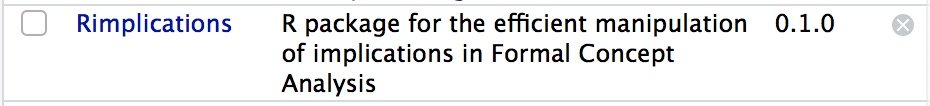
\includegraphics[scale=0.75]{docs1}
    \caption{Ejemplo Documentaci\'on 1}
    \label{fig:docs1}
\end{figure}

\begin{figure}[H]
    \centering
    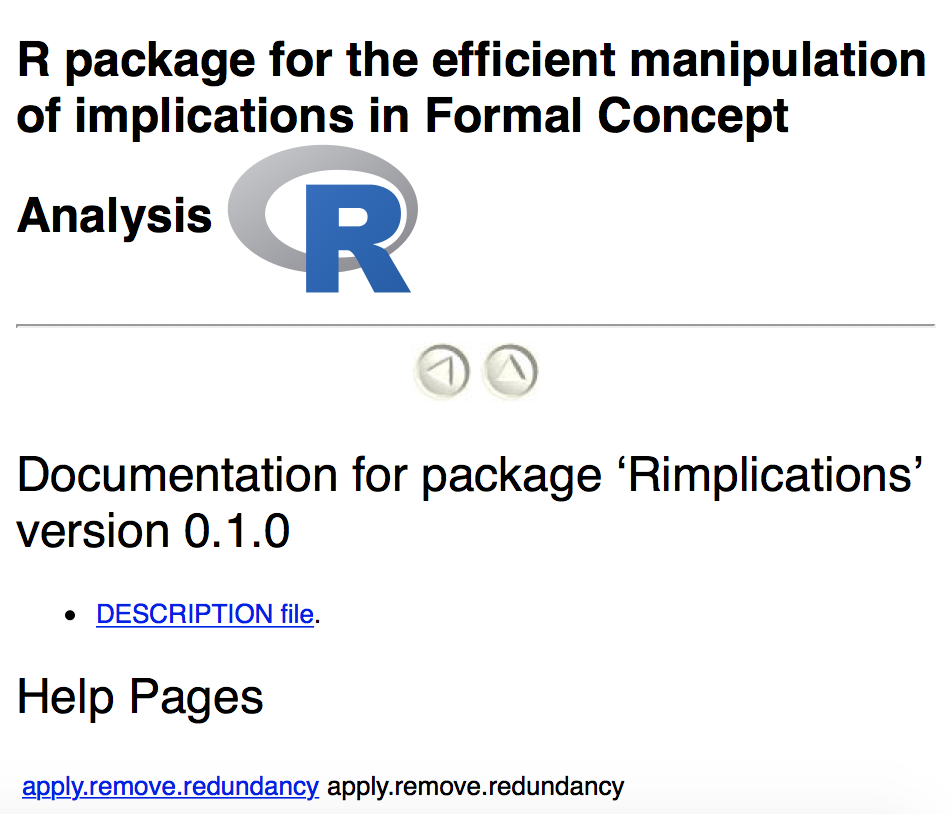
\includegraphics[scale=0.6]{docs2}
    \caption{Ejemplo Documentaci\'on 2}
    \label{fig:docs2}
\end{figure}

Aqu\'i se ve la documentaci\'on del algoritmo para la eliminaci\'on de redundancia:
\begin{figure}[H]
    \centering
    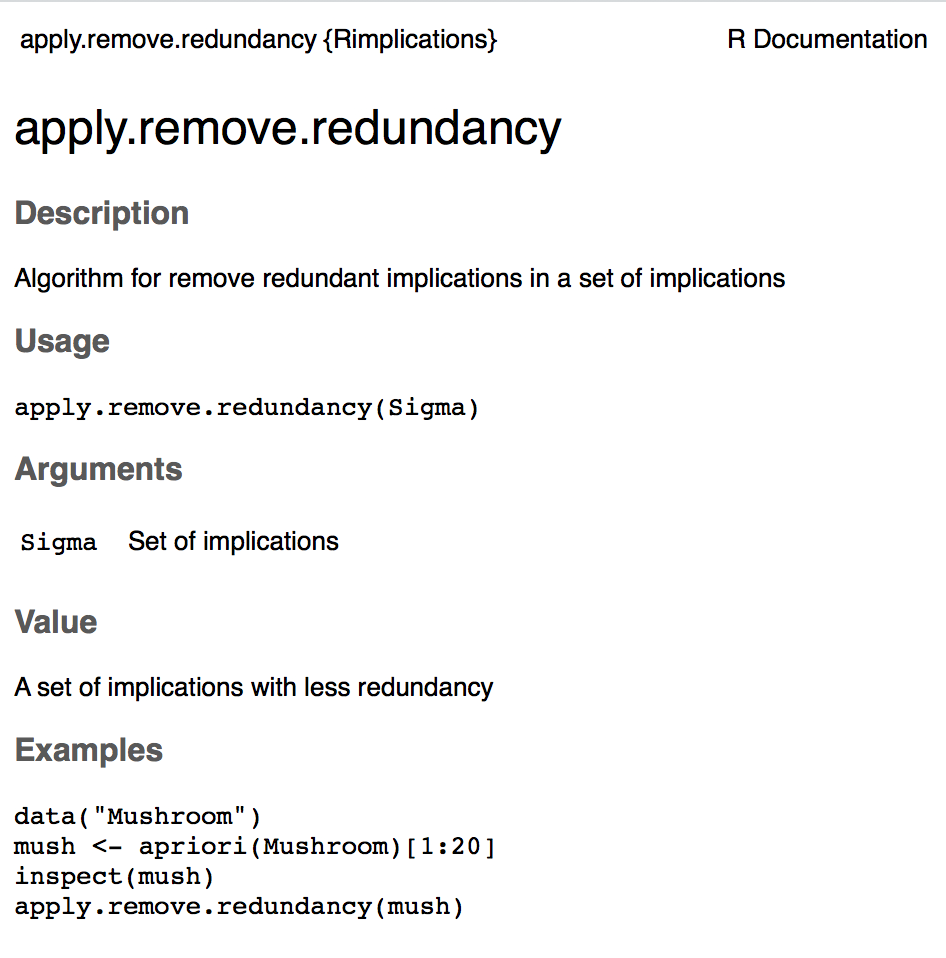
\includegraphics[scale=0.75]{docs3}
    \caption{Ejemplo Documentaci\'on 3}
    \label{fig:docs3}
\end{figure}
\newpage
\bibliographystyle{unsrt}

\bibliography{Bibliografia2} 




\end{document}